%!TEX root = ../report.tex
\section{Taktik}

\subsection{Begriffe \& Systematik}
\begin{description}
  \item[Taktik] ist ein System von Handlungsplänen und Entscheidungsalternativen, das Trainings- und Wettkampfverhalten so zu regulieren gestattet, dass ein optimaler sportlicher Erfolg möglich wird.
  \item[Strategie] ist über längere Zeit gesehene Taktik.
\end{description}
\begin{figure}[H]
  \begin{flushleft}
    \textbf{Systematisierung nach Zeit}
  \end{flushleft}
  \centering
  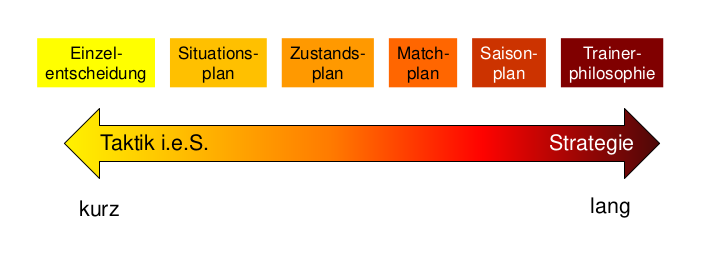
\includegraphics[width=.7\textwidth]{pictures/taktik_systematisierung.png}
  \caption{Systematisierung von Taktik nach Zeit}
\end{figure}
\paragraph{Systematisierung nach \# beteiligter Spieler} Taktik kann abhängig von der Anzahl der Spieler eingeteilt werden. Teilbereiche sind dann Mannschaftstaktik, Gruppentaktik und Individualtaktik.
\paragraph{Systematisierung nach Spielsituation} Mögliche Varianten sind Standardsituation, Offensivtaktik, Defensivtaktik, Übergangsphasen
\paragraph{Systematisierung nach Trainingszielen}
\begin{itemize}
  \item Taktische Kenntnisse: Wissensbestände, deklaratives Wissen
  \item Taktische Fähigkeiten: Situationsübergreifende taktische Handlungskompetenz: Wahrnehmung, Entscheidung, Ausführung
  \item Taktische Fertigkeiten: Angemessene und erfolgreiche Antworthandlungen (Individuell, teilkollektiv und kollektiv)
\end{itemize}
\paragraph{Taktische Handlungsphasen (nach Heckhausen)}
\begin{enumerate}
  \item Prädezisionale Phase: Wählen/ Entscheiden
  \item Präaktionale Phase: Planen/ Abschirmen
  \item Aktionale Phase: Ausführen
  \item Postaktionale Phase: Vergleichen/ Bewerten
\end{enumerate}
\begin{figure}[H]
  \begin{flushleft}
    \textbf{Phasenstruktur taktischen Handelns (nach Mahlo)}
  \end{flushleft}
  \centering
  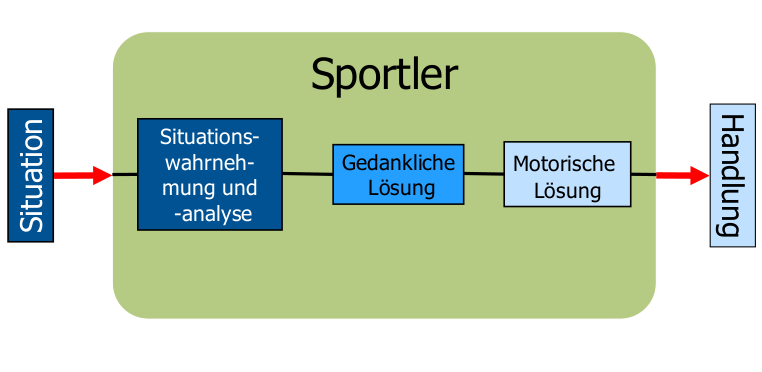
\includegraphics[width=.7\textwidth]{pictures/taktik_phasenstruktur_des_handelns.png}
\end{figure}
\paragraph{Fehlerquellen bei taktischen Entscheidungen} Taktische Fehlentscheidungen können durch alle 3 Phasen enstehen. Falsche Situationswahrnehmung und -analyse (sensorische Probleme), Inkorrekte gedankliche Lösungen (Wahl der falschen Alternative, Menge an Vorerfahrung, akt. Einflüsse) und eine mangelnde motorische Umsetzung (Fehleinschätzung der Fähigkeiten, situative Umstände)


\subsection{Determinanten}

\subsection{Trainingsmethoden}

\subsection{Trainingsinhalte}

\subsection{Anwendung}

\subsection{Diagnostik}

\subsection{Zusammenfassung}
